\documentclass[]{report}   % list options between brackets
\usepackage[T1]{fontenc}
\usepackage{xcolor}
\usepackage{listings}
\lstset
{ %Formatting for code in appendix
    %basicstyle=\footnotesize,
    % line number stuff
    numbers=left,
    stepnumber=1,
    xleftmargin=4.0ex,
    showstringspaces=false,
    tabsize=4,
    breaklines=true,
    breakatwhitespace=false,
}
\usepackage[titletoc]{appendix}
\usepackage{graphicx}
\usepackage{textcomp}
\lstset{basicstyle=\ttfamily,
  showstringspaces=false,
  commentstyle=\color{red},
  keywordstyle=\color{blue}
}
\usepackage[utf8]{inputenc}
\usepackage[english]{babel}
 
\usepackage{hyperref}
\hypersetup{
    colorlinks=true,
    linkcolor=blue,
    filecolor=magenta,      
    urlcolor=cyan,
}
 
\usepackage{pythonhighlight}
% \usepackage{ipython}
\usepackage{courier}
% type user-defined commands here


\definecolor{titlebgdark}{RGB}{0,163,243}
\definecolor{titlebglight}{RGB}{191,233,251}

%\usepackage{mystyle} % Nannas hacks
\usepackage{enumitem}
\usepackage[backend=bibtex8]{biblatex}
\bibliography{report.bib}
\begin{document}
\sloppy

					
\lstset{language=python,upquote=true}
\setlist[enumerate]{itemsep=0mm}
\setlist[itemize]{itemsep=0mm}
\setlength\parindent{0pt}

%-------------------------------------------------------------------------------
% TITLE PAGE
%-------------------------------------------------------------------------------
\begin{titlepage}
    \begin{center}
        \vspace*{1cm}
        \Huge
        \textbf{WeBook}
        
        \vspace{0.5cm}
        \LARGE
        Convert a Webpage to an E-book
        
        \vspace{1.5cm}
        \textbf{By: Jan Christian Refsgaard}
        
        \vfill
        \vspace{0.8cm}
        
        \Large
        Student ID: S124517 \\
        Subject: 62T04 Web Technologies E17 \\
        Teacher: Birger Andersen, birad@dtu.dk \\
        Date: 20/12-2017 \\
        Key strokes: 30157\\
        % pbpaste |tr -d '[:space:] ' | wc -c
        
    \end{center}
\end{titlepage}

% \maketitle

%-------------------------------------------------------------------------------
% TABLE OF CONTENTS
%-------------------------------------------------------------------------------
\tableofcontents

%-------------------------------------------------------------------------------
% ABBREVIATIONS
%-------------------------------------------------------------------------------
\chapter*{Abbreviations}
\begin{tabular}{ l l }
	\textbf{CDN}   & \textbf{C}ontent \textbf{D}istribution \textbf{N}etwork  \\
	\textbf{EPUB}  & \textbf{E}lectronic \textbf{PUB}lication  \\
	\textbf{HTML}  & \textbf{H}yper\textbf{T}ext \textbf{M}arkup \textbf{l}anguage \\
	\textbf{HTML5} & \textbf{H}yper\textbf{T}ext \textbf{M}arkup \textbf{l}anguage 
					 version 5 \\
	\textbf{OEBPS} & \textbf{O}pen \textbf{EB}ook \textbf{P}ublication \textbf{S}tructure \\
	\textbf{TOC}   & \textbf{T}able \textbf{O}f \textbf{C}ontent  \\
	\textbf{URI}   & \textbf{U}niform \textbf{R}esource \textbf{I}dentifier \\
	\textbf{URL}   & \textbf{U}niform \textbf{R}esource \textbf{L}ocator \\
    \textbf{WSGI}  & \textbf{W}eb \textbf{S}erver \textbf{G}ateway \textbf{I}nterface \\
	\textbf{XHTML} & \textbf{E}xtensible \textbf{H}yper\textbf{T}ext \\
\end{tabular}

%-------------------------------------------------------------------------------
% INTRODUCTION
%-------------------------------------------------------------------------------
\chapter{Introduction}           
Many aspiring authors publish their work on as a WordPress blog, two
of my favorite books are only available this way:
\begin{itemize}
	\item Worm\cite{worm}: \url{parahumans.wordpress.com/}.
	\item From The New World\cite{from_the_new_world}: \url{shinsekai.cadet-nine.org/} 
\end{itemize}
There are other webpages such as \url{fanfiction.net} where users have uploaded millions of books.

Because the above books are only available as websites they cannot be consumed
from an e-book reader. Nor can they be enjoyed when internet is unavailable such
as on an air plane.

\section{Problem Statement}
How can a website be converted to an e-book?

This question can be further broken down to:
\begin{itemize}
    \item how do you scrape a website
    \begin{itemize}
        \item do you have to write a scraper for each website?
		\item or can the software be made more generic?
    \end{itemize}
    \item which e-book format resemble a website most?
    \item should the software support multiple e-book formats?
    \item How do we make the tool user friendly.
\end{itemize}

\subsection{Scope}
Many e-book format exists, but EPUP is based on html, and therefore the easiest
to support when the source book is also HTML. I will not support other formats
as Calibre\cite{calibre}, support conversion between most
e-book formats.

As there are a plethora of different webpage books, that all will be needed to
be converted to EPUP, I will only write a scraper for \url{fanfiction.net}, but
strive to make the code modular so it is easy for tech savvy users to write a
parser, to further facilitate the expansion of the tool, the code is available
on github under \url{https://github.com/jancr/webook} under the MIT licence. 

To make the tool available I will make a website, as well as a command-line
interface.

My Hope is for my tool to be used by other readers and programmers. Thus to
make installation as easy as possible I will strive to mostly use functions
from Pythons standard library.

%\subsection{Methods}

%-------------------------------------------------------------------------------
% THEORY
%-------------------------------------------------------------------------------
\chapter{Theory}
\section{Electronic Publication (EPUB)}
\subsection{EPUB History}
EPUB is the successor of the Open eBook Publication Structure (OEBPS) version
1.2. For this reason the first version of EPUB, version 2.0, was released in
2007. In 2010 it reached maturity and the final specification EPUB 2.0.1 was
released \citation{epub201}. This promptet the development of version 3 where there
is still active development\cite{epub301}. The Difference between the 2.0 and
3.0 mostly new features such as support for mathML and support for Fixed Layout
Documents such as comments\cite{epub2to3}. Also version 2.0 uses XHTML where
version 3.0 supports both XHTML and HTML5. EPUB 3.0.1 is mostly backwards
compatible with 2.0.1\cite{epub2to3}. 

\subsection{Implementation}
As many e-book readers have different screen sizes, the standard has opted to
use HTML + css, to facilitate reflowable documents.

An EPUB is basically a website, contained in a ZIP archive. To see this lets download a public domain book (Listing \ref{lst:download-metamorphosis}). Please note that I am using the back tick hack to split the url over multiple lines.

\begin{minipage}{\linewidth}
\begin{lstlisting}[language=bash, label={lst:download-metamorphosis}, 
				   caption={Downloading and unzipping an ebook}]
wget "https://s3-us-west-2.amazonaws.com/"`
     `"pressbooks-samplefiles/MetamorphosisJacksonTheme/"`
     `"Metamorphosis-jackson.epub"
unzip Metamorphosis-jackson.epub
\end{lstlisting}
\end{minipage}

Which yields the output shown in Listing \ref{lst:ls-metamorphosis}:

\begin{minipage}{\linewidth}
\begin{lstlisting}[language=bash, label={lst:ls-metamorphosis}, 
				   caption={Metamorphisis EPUB file structure}]
Archive:  Metamorphosis-jackson.epub
 extracting: mimetype
  inflating: toc.ncx
  inflating: OEBPS/chapter-001-chapter-i.html
            ...
  inflating: OEBPS/jackson.css
  inflating: book.opf
  inflating: META-INF/container.xml
  inflating: META-INF/com.apple.ibooks.display-options.xml
\end{lstlisting}
\end{minipage}
% removed from ...
  % inflating: OEBPS/chapter-002-chapter-ii.html
  % inflating: OEBPS/title-page.html
  % inflating: OEBPS/front-cover.html
  % inflating: OEBPS/chapter-003-chapter-iii.html
  % inflating: OEBPS/copyright.html
  % inflating: OEBPS/table-of-contents.html
  % inflating: OEBPS/assets/pressbooks-promo.png
  % inflating: OEBPS/assets/MedulaOne-Regular.ttf
  % inflating: OEBPS/assets/themetamorphosis_1200x1600.jpg
  % inflating: OEBPS/pressbooks-promo.html

We see above that the website aspects of the e-book is located in the folder
\texttt{OEBPS}, while this is not mandatory, it is common practice, the folder
is named \texttt{OEBPS} because it is the predecessor to EPUB.

Apart from the website aspects of \texttt{Metamorphosis-jackson.epub} where all
the chapters are located, there three other files mandated by the EPUB
standard\cite{epub301}:
\begin{itemize}
	\item \texttt{META-INF/container.xml} This XML file points to the file \texttt{*.opf} file(s)
    \item \texttt{book.opf}: Open Package Format (URI:
          \url{http://www.idpf.org/2007/opf}), a file containing meta data, such as
          author name, and a manifest indexing the books content, in this case all
          the files in the OEBPS folder.
    \item \texttt{toc.ncx} The table of context, an XML file (URI:
          \url{http://www.daisy.org/z3986/2005/ncx/}.
\end{itemize}

\section{Python 3}
\subsection{Quick Python Intro for Programmers}
Python is one of the easiest languages to learn. The standard hello world is
only one line (see Listing \ref{lst:hello-world})

\begin{minipage}{\linewidth}
\begin{lstlisting}[language=python, label={lst:hello-world}, 
                   caption={Python hello world}]
print("hello world")
\end{lstlisting}
\end{minipage}

Python uses whitespace to signify end of code block, thus all code that have
the same indentation are in the same block. This avoids the dangling else
problem\cite{dangling_else} as can be seen in Listing \ref{lst:dangling-else}

\begin{minipage}{\linewidth}
\begin{lstlisting}[language=python, label={lst:dangling-else}, 
                   caption={Python: no dangling else}]
y = x = 2
if y == 3:
    if x == 3:
        print('x is 3')
else:  # the else belongs to the if with the same indentation
    print('y is not 3')
\end{lstlisting}
\end{minipage}

Python 3 is under rapid development, and in version 3.6 f strings were
introduced, allowing you to seamlessly intermingle code and strings, by
prepending stings with an \textbf{\texttt{f}}, you can run arbitrary python
code between \{ and \} as exemplified in Listing \ref{lst:f-strings}

\begin{minipage}{\linewidth}
\begin{lstlisting}[language=python, label={lst:f-strings}, 
                   caption={Python: f strings}]
x = 'hat,cat'
print(my f"{x.split(',')[0]} is beautiful")
# prints "my hat is beautifull"
\end{lstlisting}
\end{minipage}

For a more in depth tutorial the tutorial at \url{
https://docs.python.org/3/tutorial/index.html} is excellent.

%\subsection{OOP}
\subsection{Web Scraping}
Web scraping refers to the act of extracting data from a website, it can be
done manually, but most often it is done programmatically. As crawling a server
risks overloading it, many pages have a file named
\texttt{robots.txt}\cite{robots} that specifies, which parts of the site robots
are allowed to scrape. Of course malicious bots can simply ignore \texttt{robots.txt}. 

There are many different tools and libraries that can assist one. The most
simple way to scrape a website is simply to make GET requests to web pages,
find links, and then make GET requests to those. While this works wonders for
static pages, it falls short on dynamic web pages. For very dynamic websites where
JavaScript needs to be interpreted for the site to load.
Scraping libraries like Java's HtmlUnit, "a GUI less browser for Java
Programs"\cite{java_htmlunit} can be used to scrape dynamic pages. There is also
Selenium\cite{selenium} which is often used for front end testing by automating
a browser. There is even python bindings for selenium\cite{py_selenium}.

Luckily \url{fanfiction.net} and similar pages are not very dynamic, making
the request functions from the python standard library sufficient.

\subsection{Flask}
Flask\cite{flask} is a microframework, it is thus very lightweight and ideal for small
web pages. It builds upon two other python packages. 1. Werkzeug, a WSGI (Web
Server Gateway Interface). 2) Jinja 2, a templating language that allows you to
mix python and html, much like php.

Much like python, hello world in Flask (see Listing
\ref{lst:flask-hello-world}) is also surprisingly few lines. 

\begin{minipage}{\linewidth}
\begin{lstlisting}[language=python, label={lst:flask-hello-world}, 
                   caption={Flask Hello World}]
import flask
app = flask.Flask(__name__)

@app.route("/")
def hello():
    return "Hello World!"
\end{lstlisting}
\end{minipage}

\textbf{Line 1-2:} Imports Flask, and instanciates the WSGI server \\
\textbf{Line 4:} this decorator\cite{py_decorator} assigns the '/' request (both GET and POST) to
the function \texttt{hello} \\
\textbf{Line 5-6:} a Python functio that returns "HTTP/1.1 200 OK" with "Hello
World" as data \\

If instead of returning plain text we want to return html, then we need two
things, 1. A Jinja 2 template which is html interlaced with python code, much
like a php script can be a mixture of php code and html 2. We need the function
\texttt{flask.render\_template}, that takes a Jinja 2 template as argument and
processes it into html. Much like the PHP interpreter does with \texttt{*.php} files.

\subsubsection{Jinja 2}
The base idea of Jinja is that you create one base template, and extend it,
data is passed to the template via \texttt{render\_template}. Listing
\ref{lst:jinja-example} shows an example Jinja 2 template.

\begin{minipage}{\linewidth}
\begin{lstlisting}[language=python, label={lst:jinja-example},
                   caption={Jinja 2 example}]


  <ul>
  
    <li><a href="{{ user.url }}">{{ user.name }}</a></li>
  
  </ul>

\end{lstlisting}
\end{minipage}

Here is a brief walk trough of the code in Listing \ref{lst:jinja-example}: \\
\textbf{Line 1:} This an extension of another Jinja 2 template \texttt{layout.html} \\
\textbf{Line 2 and 8:} The following code goes into the 'body' block of
\texttt{layout.html} \\
\textbf{Line 4-6:} python code is encapsulated in \texttt{\{\% \%\}} and python
variables in \texttt{\{\{ \}\}}

Assuming the above template in Listing \ref{lst:jinja-example} is called
\texttt{users.html} and you want to pass it the variable \texttt{all\_user},
then \texttt{render\_template} would be called with two arguments, 1. The
template (\texttt{users.html}, and 2. The user variable(\texttt{all\_user})

\begin{minipage}{\linewidth}
\begin{lstlisting}[language=python, label={lst:render-template},
                   caption={Flask render\_template, renders a Jinja 2 template}]
@app.route("/users.html")
def users():
    return flask.render_templates('users.html', 
                                  user=all_user)
\end{lstlisting}
\end{minipage}

\subsection{Concurrent Programming and Parallelism}
\label{sec:concurrent_programming}
Concurrent programming and parallelism are two different strategies for
speeding up code. An example of parallelism is multi threading or
multiprocessing where a subset of the problem is handled to each given to a
worker. If however the majority of time is not spend doing computations but by
waiting on blocking calls such as waiting for a HTTP request or IO on the file
system, a substantial speed up can be achieved by scheduling other parts of the
program to run while waiting.

In Python multi threading will speed up blocking programs, but it will not
speed up non blocking programs as only one thread can be scheduled to run
inside the interpreter. In python 3.5 a new syntax (\texttt{asyng/await})
became available for concurrent programming without threads, this is a very
interesting development for the language, but as of writing this is only
supported for HTTPS/DNS using external libraries such as \texttt{aiohttp}. 

In python 3.2 a new library
\texttt{concurrent.futures}\cite{py_concurrent_futures} became available, which
makes it easy to switch between multi processing and multi threading code. By
providing the same API for both. As this library is part of the std library it
is the preferred way to concurrent make GET/POST requests. Interesting the
developers of \texttt{async/await} also named their concurrency object
\texttt{Future}, and gave them a very similar API, making it somewhat easy to
switch code from one paradigm into the other. 


%-------------------------------------------------------------------------------
% WEBOOK 
%-------------------------------------------------------------------------------
\chapter{WeBook}
WeBook is short for Web page to e-book. It is a framework that as the name
implies facilitates conversion of a webpage to an ebook. It is written in pure
python, except for it's front end which is written in html and JavaScript.

\section{Overwiev}
Weebook has 3 main components:
\subsection{User Interface}
\begin{figure}[h]
    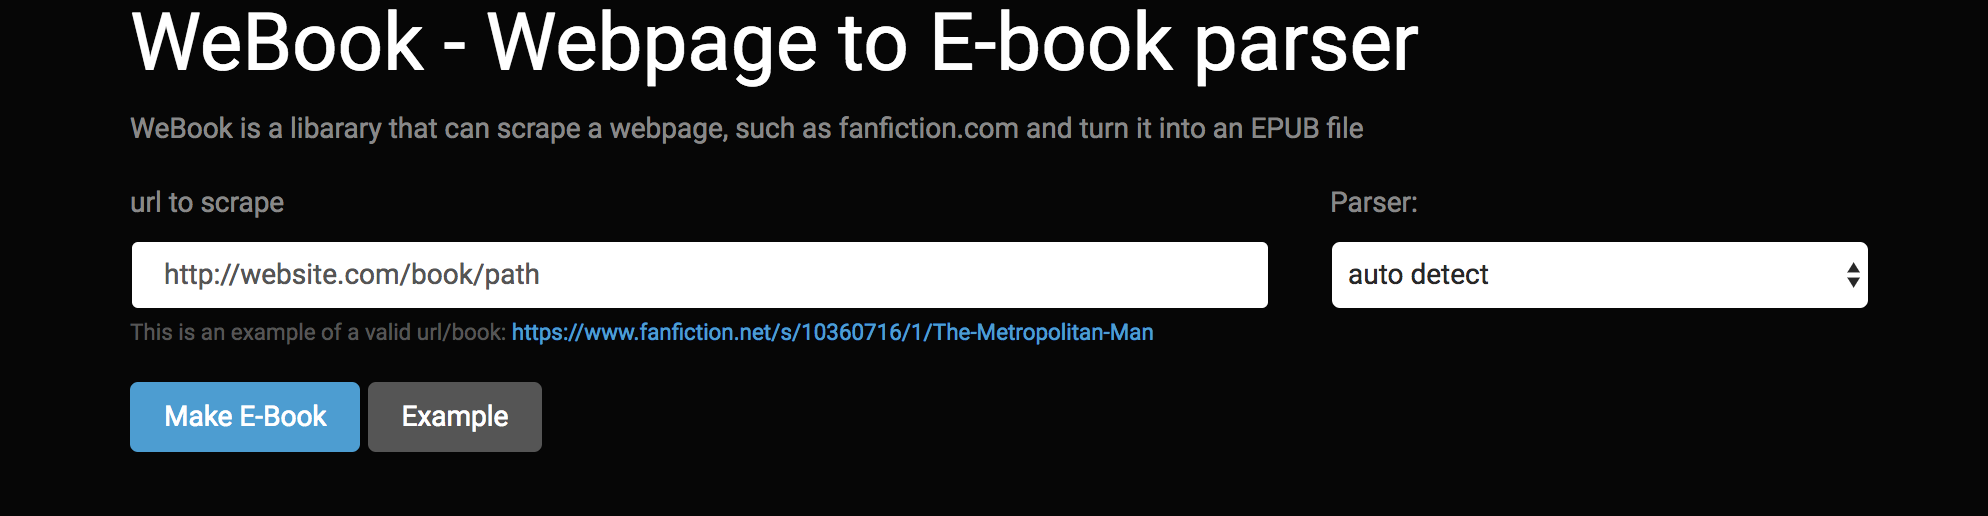
\includegraphics[width=\textwidth]{img/webook_web.png}
    \caption{Screen Shot of the WeBook web interface}
    \label{fig:webook-web}
\end{figure}

There are two ways to interact with webook, it can be invoked as a command line tool (run \texttt{webook -h} or read the projects README for more information)

The second way to use WeBook is by interacting with its webserver:
\begin{itemize}
    \item A web server that can be started by the command:
    \begin{itemize}
        \item \texttt{webook --webserver}
    \end{itemize}
    \item once started, the web server (shown in Figure \ref{fig:webook-web})
        is running on localhost port 5555 (\url{http://0.0.0.0:5555/}
    \item simply copy a book url from fanfiction into the "url to scrape" input box, or click "Example"
    \item click submit and wait for your book
\end{itemize}

\subsection{E-Book Generator}
The core of The e-book is the class \texttt{EBook} where all the code to create
an e-book resides. It is written as a class who's subclasses are tasked with
the scraping of specific websites. For more information, the source code for
\texttt{EBook} is located in \texttt{webook/webook.py}. And Section
\ref{sec:ebook} documents the class in depth.

\subsection{Web Scraper}
The subclasses of \texttt{EBook} are tasked with doing the scraping of
web pages, and turning the scraped text into an e-book using the inherited
methods from it's parent. Currently only 1 subclass exists
(\texttt{FanfictionEBook} in \texttt{webook/modules/fanfiction.py}), but as it
is only 33 lines of code, it should not be to big of a burden to create more.
For more information please read section \ref{sec:FanFictionEBook}

\section{Install Instructions}
First Install Python (\url{https://www.python.org/downloads/})

Then clone WeBooks git repository and run the installer using \texttt{pip} (the
python package installer), thise commands are shown in Listing
\ref{lst:install}. This will install all the dependencies for WeBook as well as
webook itself. 

\begin{lstlisting}[language=bash, label={lst:install},
                   caption={WeBook install instructions}]
git clone https://github.com/jancr/webook.git
cd webook
pip3 install setup.py
\end{lstlisting}

to uninstall webook (and all it's dependencies) run the commands in Listing \ref{lst:uninstall}
\begin{lstlisting}[language=bash, label={lst:uninstall},
                   caption={WeBook uninstall instructions}]
pip3 uninstall webook
pip3 uninstall beautifulsoup4
pip3 uninstall lxml
pip3 uninstall tqdm
pip3 uninstall flask
\end{lstlisting}

\section{Design and Technology Choices}
\subsection{E-book format}
Because of EPUB 3.0.1 is mostly backwards compatible with EPUB
2.0.1\cite{epub2to3} and because the EPUB 2.0.1 specification is simpler, I have
opted for creating EPUB that conform to both standards. This is achieved by
using XHTML instead of HTML5.

\subsection{Python and Libraries}
To keep the project simple, I have opted to use the same language (Python) for:
scraping the web-pages, creating the e-book, exposing the command line
interface and creating web server.

\textbf{E-Book generation}: As the EPUB is a mixture of xhtml and xml, a xml
parsing library is needed. The two best candidates are \texttt{ElementTree}
from the standard library or the extenal library \texttt{lxml}. They both have
very similar syntax, and \texttt{ElementTree} is basically a subset of
\texttt{lxml}. I don't strictly need any of the features from \texttt{lxml}
though it's handling of name spaces is better than \texttt{ElementTree}.

\textbf{Web scraping}: There are many good python libraries that can simplify the for web-scraping.
\begin{itemize}
    \item \textbf{\texttt{mechanize}:} Which has a very natural and powerful API
    \item \textbf{\texttt{urllib}:} Part of the Python standard library, can make GET requests.
    \item \textbf{\texttt{requests}:} One of the most popular Python libraries,
        has better API than urllib, but is not part of the standard library
	\item \textbf{\texttt{selenium}}\cite{py_selenium}: Python bindings for the popular Selenium\cite{selenium}
    \item \textbf{\texttt{Beautiful Soup}:} Prominent html Parsing library
\end{itemize}
As I have a commitment to keeping the number of dependencies low I will parse
urls and make requests using \texttt{urllib} from the standard library. But as
many web pages can be malformed I need a mature library, that parses html much
the same way as the browser, and have thus settled on \texttt{Beautiful Soup}.
Interesting \texttt{Beautiful Soup} uses \texttt{lxml} as it's html parser. So
my code indirectly depend on \texttt{lxml}.

\section{Code and File Structure}
%\subsection{EPUB Files}
The base idea is that for each book type (EPUB, MOBI etc), the base skeleton
will be available under \texttt{webook/book\_templates}, for now only EPUB is
available (\texttt{webook/book\_templates/epub\/}).

% \begin{lstlisting}[language=bash,basicstyle=\small]
% $ ls -lh book_templates/epub/*
% -rwxr-xr-x  1 jcr  staff   934B Nov 22 12:23 content.opf
% -rwxr-xr-x@ 1 jcr  staff    20B Jun  4 23:19 mimetype
% -rwxr-xr-x@ 1 jcr  staff    50B Jun  4 23:19 page_style.css
% -rwxr-xr-x@ 1 jcr  staff   404B Jun  4 23:19 page_template.xhtml
% -rwxr-xr-x@ 1 jcr  staff   670B Jun  4 23:19 titlepage.xhtml
% -rwxr-xr-x  1 jcr  staff   578B Nov 22 17:40 toc.ncx
% 
% META-INF:
% -rwxr-xr-x@ 1 jcr  staff   225B Nov 22 19:06 container.xml
% \end{lstlisting}
% 
\subsection{Static Files}
Here I will describe all the files that are hard coded, and thus not changed by the code. 

\texttt{mimetype} specifies the EPUP mimetype (\texttt{application/epub+zip}).
\texttt{META-INF/container.xml} points out where the root file is located, it
is hard coded to point to \texttt{content.opf}. \texttt{page\_style.css}
contains the css to style the book. While I could allow the parser to also
scrape style sheets, I think it is better to hard code it as some pages may
have the style sheet cascade in such a way that they are not applied correctly,
when only a small portion of the web page is scraped.

\subsection{content.opf}
The \texttt{content.opf} is an xml file with two important tags
\begin{itemize}
    \item \texttt{<metadata>}, such as cover image, author name and book title.
    \item \texttt{<manifest>}, a reference to every file that needs to be
        indexed, it is hard coded to have references to \texttt{titlepage.xhtml}, \texttt{page\_style.css} and \texttt{toc.ncx}. Each chapter scraped should result in an xhtml file with an entry here.
\end{itemize}

\subsection{toc.ncx}
Contains the Table of Content. This file contains two important tags: 
1. \texttt{<docTitle>}: where you put the title of the book
2. \texttt{<navMap>}, an xml structure that specifies the nesting of book
sections and "read order" (\texttt{playOrder}). Listing \ref{lst:toc} shows
the xml WeBook generated for a simple 1 page story.

\begin{minipage}{\linewidth}
\begin{lstlisting}[language=XML, label={lst:toc}, 
                   caption={toc.ncx example <navMap>}]
<navMap>
    <navPoint id="navPoint-1" playOrder="1">
        <navLabel><text>Etcetera</text></navLabel>
        <content src="titlepage.xhtml"/>
    </navPoint>
    <navPoint id="navPoint-2" playOrder="2">
        <navLabel><text>Etcetera</text></navLabel>
        <content src="short_story.xhtml"/>
    </navPoint>
  </navMap>
\end{lstlisting}
\end{minipage}

If the \texttt{navPoints} in Listing \ref{lst:toc} were nested deeper, then the
EPUBs TOC would likewise be nested.

\subsection{EBook}
\label{sec:ebook}
This class (located in \texttt{webook/webook.py} contains all the logic needed
to create an Ebook. It has one very important abstract method \texttt{scrape}
that all subclasses should implement to scrape web pages.

\subsubsection{High Level Overview}
The EBook class does the following:

\begin{itemize}
	\item moves all files from \texttt{book\_templates/epub} to a temporary directory
	\item creates datastructures to manipulate the \texttt{content.opf} and \texttt{toc.ncx} xml files
	\item calls the abstract method crawl, 
	\begin{itemize}
		\item  This method should crawl the target site, and (if possible) set
			\texttt{self.title}, \texttt{self.first\_name} and \texttt{self.last\_name} (of the author), and
			\texttt{self.cover\_path} (to add a cover image).
		\item for each book chapter/section/arch etc. created
			\texttt{self.write\_html} needs to be called to write the chapter
			to file, and \texttt{self.update} needs to be called to update the
			\texttt{content.opf} and \texttt{toc.ncx} data structures.
	\end{itemize}
		\item dumps the updated \texttt{content.opf} and \texttt{toc.ncx} to disk. 
		\item create a zip archive of the temporary directory and give it the \texttt{.epub} extension
		\item delete the temporary directory
\end{itemize}

\subsubsection{Documenting Key Methods}
\textbf{The constructor} (\texttt{\_\_init\_\_}) takes the following arguments:
\begin{itemize}
	\item \texttt{url}: The website to scrape
	\item \texttt{epub\_file}: The filename of the ebook generated
	\item \texttt{title}: The title of the book, if not None, it overwrites the scraped book name.
	\item \texttt{workers}: The max number of concurrent TCP requests
	\item \texttt{run}: Set to false if you want to create the python object without also creating the book right away, this is necessary if you want to add a status bar. 
\end{itemize}

The constructor initiates the following important objects
\begin{itemize}
	\item \texttt{output\_dir}: the path to the temporary folder, where the book will be build.
	\item \texttt{toc}: An ElementTree (xml object), to facilitate manipulation of the \texttt{toc.ncx} (Table of Content xml file)
	\item \texttt{toc\_dict}: A dictionary mapping that maps names (usually of chapters) to their table of content xml element, 
	\item \texttt{content*} a set of instance variables for easy alteration of the \texttt{content.opf} xml file.
\end{itemize}


\textbf{\texttt{run}}: This function is a generator, that \texttt{yield} the progress of
the webscraping. When it is done scraping it updates the author name, title,
and cover image. This is done after scraping is complete,
because it assumes that the scraper will set these variables as it scrapes the
webpages. Finally it calls \texttt{self.save(self.epub\_file)} create the ebook.


            % self.update_author(self.first_name, self.last_name)
% title
% (\texttt{self.update\_title(self.title)}), which it assumes was scraped by
% \texttt{self.scrape}. Then it adds a cover a cover image
% (\texttt{self.update_title(self.title)}) which it again assumes was set by
% scrape. Finally it saves the book (\texttt{self.save(self.epub_file)}).

\textbf{\texttt{save}}: This method dumps the \texttt{toc} and \texttt{content} to disk, zip the temporary folder, and renames it to \texttt{epub\_file}, subsequently it deletes the temporary directory.

\textbf{\texttt{write\_html}}: This method creates an html file corresponding to a section/chapter/etc. it takes 3 arguments:
\begin{itemize}
	\item \texttt{text} a string or Beautiful Soup tag that will be written to file.
	\item \texttt{name}, this is the name of the file on disk (with no extension), but it is also the name used to referee to it's place in the TOC. 
	\item \texttt{header} (optional): The heading, eg "Chapter 2" or "The boy who lived" or similiar, if None it will use \texttt{name} as \texttt{header}
\end{itemize}

\textbf{\texttt{update}}: This method makes the ebook "aware" that a new book segment
have been added, by updating \texttt{content} and \texttt{toc}. In previous
iterations of the tool this method was called by \texttt{write\_html}. However
when I made the code asynchronous, such that multiple book chapters can be
crawled and written concurrently I had to make this into it's own function, as
you have to update the Table of Content in order!

\subsection{FanFictionEBook}
\label{sec:FanFictionEBook}
\texttt{FanfictionEBook} is a subclass of \texttt{Ebook}. It thus implements the \texttt{scrape} method responsible for scraping all chapters from and calling \texttt{update} to add them to the Table of Content.

Organisationally \texttt{FanfictionEBook} is found under
\texttt{modules/fanfiction.py}, because architecturally parsers for other book
websites should each live in it's own file to encourage other tech savvy to
develop their own scraper, while piggy backing on \texttt{EBook} to perform all
the heavy lifting of creating an ebook. Because all the heavy lifting is done
by the parent class, \texttt{FanFictionEBook} is only 33 lines of code
(ignoring blank lines). 

\begin{minipage}{\linewidth}
\begin{lstlisting}[language=python, caption={FanFictionEBook.scrape}, escapeinside={(*}{*)}, 
                   label={lst:ff-parse}, basicstyle=\small]
options = select.find_all('option') (*\label{code:ff-scrape-option}*)
url_chapters = range(1, len(options)+1) (*\label{code:ff-scrape-url}*)
self.total = len(url_chapters)  (*\label{code:ff-scrape-total}*)
with futures.ThreadPoolExecutor(max_workers=workers) as executor: (*\label{code:ff-scrape-with}*)
    _exe = executor.map(self.parse_chapter, options, repeat(book_id), url_chapters) (*\label{code:ff-scrape-map}*)
    for self.progress, (file_name, chapter_name) in enumerate(_exe, 1): (*\label{code:ff-scrape-for}*)
        self.update(file_name, chapter_name) (*\label{code:ff-scrape-update}*)
        yield self.progress (*\label{code:ff-scrape-yield}*)
\end{lstlisting}
\end{minipage}

As mentioned in \ref{sec:concurrent_programming} When performing blocking
programming concurrency can speed up the process. This is a achieved by using a
the \texttt{TreadPoolExecutor} object. The code in Listing \ref{lst:ff-parse} shows how these are used.
\begin{itemize}
	\item Line \ref{code:ff-scrape-option} captures the \texttt{<option>} tags within a \texttt{<select>} tag. Thise options contains links to all the other chapters.
	\item Line \ref{code:ff-scrape-url} creates a list of numbers corresponding to the chapters, this is later used by the helper method \texttt{parse\_chapter} because the link for each chapter is:
		\begin{itemize}
			\item \texttt{https://www.fanfiction.net/s/BOOK\_ID/CHAPTER\_NUMBER}
		\end{itemize}
	\item Line \ref{code:ff-scrape-total} sets the instance variable total such that status bars are aware how many chapters needs to be scraped in total.
	\item Line \ref{code:ff-scrape-with} creates a with block, within this
		block the executor object can be used to spawn multiple threads in
		parallel. 
	\item Line \ref{code:ff-scrape-map} the executor object is used to map the
		\texttt{self.parse\_chapter} method to the arguments needed to download
		the chapters. These threads return a \texttt{future} which is
		special python object. 
	\item Line \ref{code:ff-scrape-for} Iterates over the future
		\texttt{\_exe}. The \texttt{map} and \texttt{for} combination used here
		iterate over the futures in the order with which they are submitted.
		Thus if chapter 4 is downloaded before chapter 3, the for loop will
		block until chapter 3 is received. 
	\item Line \ref{code:ff-scrape-update} calls \texttt{self.update} the
		method responsible for updating the Table Of Content. It is of course
		very important that chapters are added to the TOC in the correct order,
		which is why the \texttt{for} and \texttt{map} syntax was chosen.
	\item Line \ref{code:ff-scrape-yield} yields the progress back to the
		caller. The result being that the flow can jump between the caller and
		\texttt{scrape}.  This is utilized to get the status bar to work. Focus
		is given back to scrap calling \texttt{next} on it. See Section
		\ref{sec:backend} and the accompanying code snippet in Listing
		\ref{lst:create_ebook} 
\end{itemize}

\subsection{Webserver}
The web server uses Flask as the back end, and JQuery + Bootstrap as the front
end. The expected path through the server is the following:
\begin{itemize}
	\item a request to '/' returns the index page \texttt{static/index.html}.
		Where the user enters the url a to an E-Book, and selects a parser
		(Only fanfiction.net is implemented as of writing).
	\item When Submit is clicked. JavaScript opens a stream to the server,
		the "stream request" hands the url and parser to the back end.
	\item the back end starts scraping the chapters, for each chapter downloaded
		the progress is feed back to client, where it it is used to update the
		progress bar.
	\item When all chapters have been crawled The server saves the file to
		disk, and sends the name of the file name back to trough the stream.
	\item This prompts the client to close the stream, and make a new request
		\texttt{/download\_ebook/<file-name>} to download the file.
	\item The server cleans up all but the newest $processes\times2 + 5$ files.
\end{itemize}

\subsubsection{Front end}
To make the web page beautiful and responsive I opted for bootstrap\cite{bootstrap} with the
dark theme cyborg\cite{bootstrap_cyborg}. I wrote all the html by hand.
\texttt{WTForms}\cite{wtforms} also looked very promising, as they are Python object that
can be render into Jinja templates seamlessly. They however adding another
dependency seemed like overkill considering I only have 2 data carrying form
elements!

\subsubsection{Back end}
\label{sec:backend}
Getting the status bar to work was challenging, because it required a large
rewrites of the EBook class, The first iteration of the EBook class and it's
subclass FanFictionEBook was written in such a way that they blocked the Python
interpreter until the book was created. Which made the status bar jump from 0\%
strait to 100\%. This issue was solved by turning \texttt{Ebook.scrape} into a
generator function. This generator is returned when you call
\texttt{EBook.run()} as seen in line \ref{code:create-ebook-run} in Listing
\ref{lst:create_ebook}. The generator is advanced by calling \texttt{next} on
it, either explicitly as seen in line \ref{code:create-ebook-next}, or
implicitly by looping over it as in line \ref{code:create-ebook-for}.

\begin{minipage}{\linewidth}
\begin{lstlisting}[language=python, label={lst:create_ebook}, caption={Flask create\_ebook}, escapeinside={(*}{*)}]
@app.route('/create_ebook/<parser>/<url>')
def create_ebook(parser, url):
    def generate(ebook_parser, tmp_file):
		ebook_generator = ebook_parser.run() (*\label{code:create-ebook-run}*)
		progress = next(ebook_generator) (*\label{code:create-ebook-next}*)
        total = ebook_parser.total
        yield f"data: {round(100 * progress / total)}\n\n"
		for progress in ebook_generator: (*\label{code:create-ebook-for}*)
            yield f"data: {round(100 * progress / total)}\n\n"
        tmp_file = os.path.basename(tmp_file)
        yield f"data: file-name: {tmp_file}\n\n"
	...
    return Response(generate(ebook_parser, tmp_file), mimetype='text/event-stream')
\end{lstlisting}
\end{minipage}

\section{Testing}
As the tool is still very immature, I have not had the time to thoroughly test it.
The Core consisting of \texttt{EBook} and \texttt{FanFictionEBook} have been well tested
manually by trying to find places where they will fail. As an example Earlier
versions \texttt{FanfictionEBook} would crash when encountering a short story, because short stories
do not have a \texttt{<select>} tag pointing to the other chapters.

The web interface is much less tested, and lacks input validation. Thus if the
parser "WordPress sites" is chosen the server will crash. If an invalid URL is
given, the server will also crash. 

The site is in principle vulnerable to replay attacks, allowing the attacker
to bypass the scraping and directly make a request for a previously generated
book, which are stored in the \texttt{tmp} folder. However, if the server was
to go live I would probably need cash the ~100 most popular books anyway, to
lighten the server load.

I do sanitise the file name, so a request for the file
\texttt{../../../etc/passwd} will be truncated to \texttt{passwd}.  The server
is very vulnerable to DOS attacks as the server performs many computations per
request, and does not limit the number of requests per host.

During my testing of WeBook 2 things have stumped me:
\begin{enumerate}
    \item If the Flask worker process crashes on the server, while a
        \texttt{text/event-stream} is open, the browser will try to reestablish
        connection, sending the same request again, effectively performing a
        DOS attack against the server, as it will crash the worker again. If
        JavaScript forgets to close the stream, the browser will likewise
        assume the connection has crashed, resulting in a requests to the server
        every 5 seconds. 
    \begin{itemize}
            \item In principle this also mean that WeBook risk downloading a book
                multiple times, if the books server is slow, this could be
                mitigated by having flask start a timer and resend the previous
                progress if more than a few seconds have passed. 
            \item Furthermore I should probably wrap the generator function
                \texttt{scrape} in a \pyth{try}/\pyth{except} statement so the
                web server, can close the stream when errors occur. 
    \end{itemize}
    \item The book cover images on \url{fanfiction.net} are distributed via a
        CDN, thus to dodge a \texttt{403 Forbidden Error} I had to set the
        request header \texttt{Referer: fanfiction.net}.
\end{enumerate}


%-------------------------------------------------------------------------------
% CONCLUSION
%-------------------------------------------------------------------------------
\chapter{Conclusion}
\section{Product}
The goal was to convert a web page to an e-book. To achieve this I developed
WeBook. WeBook has 3 parts. 1) A web page/command line interface to interact
with it, 2) A \texttt{EBook} class that facilitates the creation of the e-book,
and 3) modules (subclasses of \texttt{EBook}) that facilitates the web-scraping,
As every website is different a scraper has to be written for each one. Thus a
lot of though has been put into making the API very simple such that writing
scrapers is as simple as possible. The only modules written so fare is a scraper
for \url{fanfiction.net} which is implemented in the class
\texttt{FanFictionEBook}, this class is only 33 lines of code, which suggests
that writing parsers for other web pages is much simpler, than writing the
parent class.

I decided to develop a web page as the primary interface to WeBook. To make the
web page user friendly and easy to use I opted to use JQuery\cite{jquery}
and Bootstrap\cite{bootstrap}, which gave the website a beautiful and
responsive design. For the back end I choose the micro framework
flask\cite{flask}, using the same programming language for the web server and
web scraping allowed the web server to hook into the \texttt{EBook} subclasses
and thus monitor the download progress and stream it back to to the front end,
where the information was used to update the status bar.

\section{Future Perspectives}
\subsection{User Interface}
The Website user interface is very simple. It could be expanded by allowing the
user to overwrite the defaults. Such as uploading an alternative cover image
and overwriting the title the tool scrapes. 

\subsection{WordPress}
I have tried to make a generic 'WordPress' Blog scraper. But as different Blogs
can look very different this has proven much harder than initially anticipated.
While worm\cite{worm} and From The New World\cite{from_the_new_world} visually
look very different. They have different tags and id/names for their side bar,
and on the worm site the link points to the entire chapter, where on From The
New World, the links point to the first page of the chapter and thus requires
you to follow the link to find more pages from the same chapter.

\subsection{Generic scraper}
I would love for there to be a generic scraper, where a user could input things
like the html id for the status bar, and the name of the first and last chapter
in the status bar, id of the chapter title, and the id of the chapter text,
etc. Whether this is feasible or not has yet to be determined, but it does not
have to work perfect to supply a more pleasant reading experience than reading
online. So a few false positives such as turning the about page into a chapter
is probably acceptable behaviour. 

\subsection{Tests and Validation}
I have lots of experience with Unit testing using
\texttt{pytest}\cite{py_pytest}, and would like to write tests for most of
methods in \texttt{EBook} and \texttt{FanfictionEBook} to ensure that the core
of the project is stable.  It would also like to add input validation to the
web interface, and exception handling to the back end. Of course some
integration and system test would also be nice, but that may be overkill for
such a small project.
%-------------------------------------------------------------------------------
% Appendex
%-------------------------------------------------------------------------------
\lstset
{ %Formatting for code in appendix
    numbers=none,
    breaklines=true,
    breakatwhitespace=false,
}

\begin{appendices}
\chapter{EPUB generation}
    \section{webook/\_\_init\_\_.py}
    Code that makes the \texttt{Ebook} class available in the \texttt{webook}
    name space instead of the \texttt{webook.webook} namespace. The
    \texttt{\_\_init\_\_} file also makes the folder into a python package,
    allowing subfolders to be imported with the '.' notation.
    \inputpython{../webook/__init__.py}{1}{10000}

    \section{webook/webook.py}
    This files implements \texttt{EBook} the main Class responsible for
    creating the \texttt{*.epub} file
    \inputpython{../webook/webook.py}{1}{10000}

    \section{webook/modules/\_\_init\_\_.py}
    Code that makes the modules folder into a subpackage, so it can be imported.
    \inputpython{../webook/modules/__init__.py}{1}{10000}
    
    \section{webook/modules/fanfiction.py}
    A subclass of \texttt{EBook} that can scrape fanfiction.net books.
    \inputpython{../webook/modules/fanfiction.py}{1}{10000}

    \section{book\_templates/epub}
    Here are the base files which serves as a scaffold for \texttt{EBook} to create an EPUB file.
        \subsection{META-INF/container.xml}
        \lstinputlisting{../book_templates/epub/META-INF/container.xml}

        \subsection{content.opf}
        \lstinputlisting{../book_templates/epub/content.opf}

        \subsection{mimetype}
        \lstinputlisting{../book_templates/epub/mimetype}

        \subsection{page\_style.css}
        \lstinputlisting{../book_templates/epub/page_style.css}

        \subsection{page\_templage.xhtml}
        \lstinputlisting{../book_templates/epub/page_template.xhtml}

        \subsection{titlepage.xhtml}
        \lstinputlisting{../book_templates/epub/titlepage.xhtml}

        \subsection{tox.ncx}
        \lstinputlisting{../book_templates/epub/toc.ncx}

\chapter{User Interface}
    \section{webook/command\_line.py}
    This script contains the code to start the command line interface and the web server
    \inputpython{../webook/command_line.py}{1}{10000}

    \section{webook/runserver.py}
    This script contains all Flask code.
    \inputpython{../webook/runserver.py}{1}{10000}

    \section{webook/static/webook.js}
    client side JavaScript
    \lstinputlisting{../webook/static/webook.js}

    \section{webook/static/templates}
    The Jinja 2 templates rendered by Flask
        \subsection{layout.html}
        \lstinputlisting{../webook/static/templates/layout.html}

        \subsection{index.html}
        \lstinputlisting{../webook/static/templates/index.html}

\chapter{Install Script}
    \section{setup.py}
    \inputpython{../setup.py}{1}{10000}



\end{appendices}

%-------------------------------------------------------------------------------
% Bibliography
%-------------------------------------------------------------------------------
\printbibliography

\end{document}
